\documentclass{beamer}
\usetheme{metropolis}

\usepackage{calc}
\usepackage{enumitem}
\usepackage{graphicx}
\usepackage{textcomp}
\usepackage{upquote}
\usepackage{hyperref}
\hypersetup{colorlinks = true, linkcolor = .}

\title{Alshayun: A mobile education application}
\date{March 20, 2019}
\author{Jacob Chappell}
\institute{University of Kentucky}

\begin{document}

\maketitle

\begin{frame}{Agenda}
    \tableofcontents
\end{frame}

\section{Introduction}

\begin{frame}{What is Alshayun?}
    \begin{itemize}
        \item A mobile application for delivering articles consisting of rich
            text and interactive \textbf{applet}s to \textbf{reader}s.
        \item Designed for three actors in mind (a user is any of them):
            \begin{description}[leftmargin=!,labelwidth=\widthof{\bfseries Content Author}]
                \item[Content Author] Anyone who has anything about which they
                    would like to write.
                \item[Reader] Anyone who would like to read what one or more
                    \textbf{content author}s have to say.
                \item[Developer] Anyone capable of developing \textbf{applet}s
                    and other functionality of \textbf{Alshayun} of which
                    \textbf{content author}s and \textbf{reader}s can make use.
            \end{description}
    \end{itemize}
\end{frame}

\begin{frame}{Inspiration}
    \begin{itemize}
        \item My fascination with Bézier curves led me to the Internet.
        \item I discovered the article
            \href{https://pomax.github.io/bezierinfo/}{A Primer on Bézier
            Curves} by Pomax.
        \item I was intrigued by the interactive \textbf{applet}s weaved
            seamlessly throughout the text.
    \end{itemize}
    \begin{figure}
        \begin{center}
            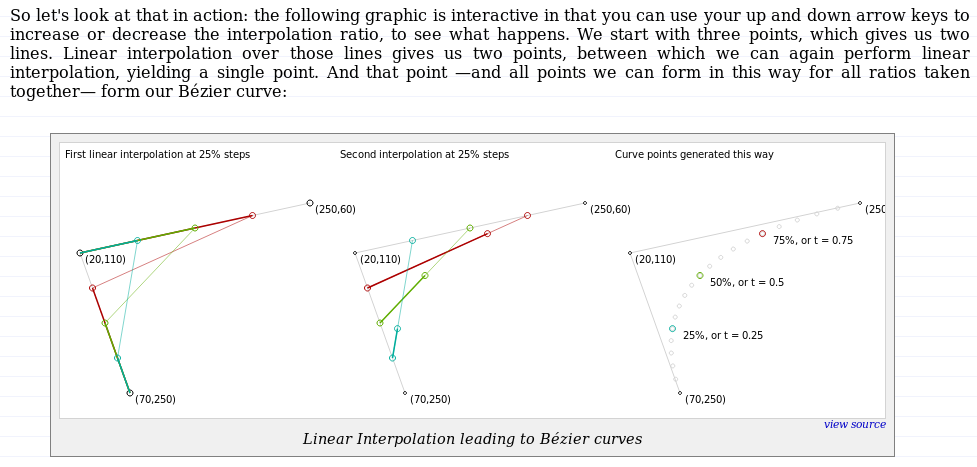
\includegraphics[scale=0.25]{images/pomax.png}
        \end{center}
        \caption{Example \textbf{applet}s from \textit{A Primer on Bézier
        Curves}.}
    \end{figure}
\end{frame}

\begin{frame}{About the Name}
    \begin{itemize}
        \item At inception, \textbf{Alshayun} was planned to be a mathematics
            education platform.
        \item I built a more general platform, but kept the original ``mathy'' name.
        \item
            \begin{center}
                \textbf{Origins of Algebra} \\
                Arabic (``al-jabr'')\textrightarrow Spanish\textrightarrow
                Latin\textrightarrow English
            \end{center}
        \item Arabic ``al-shayun'' appeared frequently in the original algebraic
            documents and means ``the unknown thing''; it became the ``x'' in
            Latin/English-speaking algebra (see
            \href{https://cosmosmagazine.com/mathematics/why-x-marks-unknown-0}{Why
            X marks the unknown} by Terry Moore).
    \end{itemize}
\end{frame}

\section{Alshayun}

\begin{frame}{User Interface}
    \begin{itemize}
        \item Live Demonstration
    \end{itemize}
\end{frame}

\begin{frame}[fragile,allowframebreaks]{Caching Strategy}
    \begin{itemize}
        \item Articles broken into two pieces: metadata and text.
        \item Metadata of all articles stored in a single manifest represented
            in \textbf{JavaScript Object Notation (JSON)} and consists of:
            \begin{description}[leftmargin=!,labelwidth=\widthof{\bfseries
                    Excerpt}]
                \item[id] A unique, monotonically-increasing integer. Used to
                    store on \textbf{reader}s device which articles have been
                    read.
                \item[title] The title of the article.
                \item[tags] Zero or more taxonomic tags.
                \item[excerpt] A short (one sentence) description of the article.
            \end{description}
        \item Text is the full article text stored separately from the manifest
            and represented in
            \href{https://daringfireball.net/projects/markdown/}{Markdown}.
    \end{itemize}
    \begin{figure}
    \begin{verbatim}
[
  {
    "id": 12,
    "title": "Tower of Hanoi",
    "excerpt": "Learn about the Tower of Hanoi...",
    "tags": [
      "algorithms"
    ]
  }
]
    \end{verbatim}
    \caption{Snippet of articles manifest in \textbf{JSON}.}
    \end{figure}
\end{frame}

\begin{frame}[fragile,allowframebreaks]{Applets}
    \begin{itemize}
        \item The crux of \textbf{Alshayun}.
        \item Implemented as \textbf{Angular} components which extend an
            \textbf{Applet} superclass.
        \item Superclass provides a \textbf{Hypertext Markup Language (HTML)}
            canvas tag and drawing context, implements an animation loop,
            provides an extensible toolbar.
        \item \textbf{Applet}s are included in articles via an \texttt{<applet>}
            \textbf{HTML} tag with extensible properties.
    \end{itemize}
    \begin{figure}
    \begin{verbatim}
<applet name="sort"
        width="50%"
        data-method="insertion"
        data-num-bars="50"></applet>
    \end{verbatim}
        \caption{Including an \textbf{applet} with an \texttt{<applet>} tag.}
    \end{figure}
    \begin{figure}
    \begin{verbatim}
@Component({
  template: appletsGenericTemplate + `
<ng-template #childToolbar>
  <a *ngIf="!doTicks && !allDone"
     (click)="doTicks = true">Play</a>
</ng-template>
  `,
  styleUrls: ['./applet.scss']
})
export class AppletSortComponent extends Applet {
    \end{verbatim}
        \caption{Snippet of the Tower of Hanoi \textbf{applet} class.}
    \end{figure}
\end{frame}

\section{Quick n' Dirty Server (QDS)}

\begin{frame}{Motivation}
    \begin{itemize}
        \item During initial development, I packaged articles into the Android
            Package (APK) file of \textbf{Alshayun}.
        \item This was a temporary solution and hindered the
            production-readiness of the application.
        \item In response, I setup an Nginx Web server on my desktop and hosted
            articles there.
        \item I wanted everything necessary to build, run, and test
            \textbf{Alshayun} to be included in the source code with detailed
            instructions.
        \item The \textbf{QDS} was born, composed of a \textbf{backend} and a
            \textbf{frontend}.
    \end{itemize}
\end{frame}

\begin{frame}[fragile,allowframebreaks]{Backend}
    \begin{itemize}
        \item Written in \textbf{Flask} and serves two functions: deliver
            articles to \textbf{Alshayun} and expose a \textbf{Representational
            State Transfer (REST)} interface to the \textbf{frontend}.
    \end{itemize}
    \begin{figure}
    \begin{verbatim}
@app.route('/articles/<path:filename>')
def get_article(filename):
    return send_from_directory('articles/', filename)
    \end{verbatim}
    \caption{\textbf{QDS} interface to serve static articles.}
    \end{figure}
    \begin{figure}
    \begin{verbatim}
@app.route('/article', methods = ['POST'])
def create_article():
    article = {}
    article['id'] = checkout_serial()
    # ... finish populating article object ...
    f = open('articles/article.' + \
        str(article['id']) + '.md', 'w')
    f.write(str(request.json['text']))
    f.close()
    # ... add article object to manifest ...
    \end{verbatim}
    \caption{Snippet of \textbf{QDS} interface to dynamically create articles.}
    \end{figure}
\end{frame}

\begin{frame}{Frontend}
    \begin{itemize}
        \item Written as a standalone \textbf{Angular} application.
        \item Communicates with \textbf{backend} via the \textbf{REST}ful
            interface the \textbf{backend} exposes.
        \item Allows creation and management of articles.
        \item Features a live preview of rendered articles as \textbf{content
            author} writes them in Markdown.
    \end{itemize}
\end{frame}

\begin{frame}{Production Considerations}
    \begin{itemize}
        \item The \textbf{QDS} is for development purposes and is not production
            ready.
        \item A real Web server (Nginx, Apache) should be configured to back the
            \textbf{frontend} and \textbf{backend}.
        \item Use a Web Server Gateway Interface (WSGI) module for interfacing
            with the \textbf{Flask} code.
        \item Secure Sockets Layer (SSL) certificates should be setup and
            utilized.
        \item Develop an authentication wall around the \textbf{REST}ful
            interface of the \textbf{backend}.
    \end{itemize}
\end{frame}

\section{Technologies Used}

\begin{frame}{Node.js}
    \begin{itemize}
        \item TODO
    \end{itemize}
\end{frame}

\begin{frame}{TypeScript}
    \begin{itemize}
        \item TODO
    \end{itemize}
\end{frame}

\begin{frame}{Angular}
    \begin{itemize}
        \item TODO
    \end{itemize}
\end{frame}

\begin{frame}{Ionic}
    \begin{itemize}
        \item TODO
    \end{itemize}
\end{frame}

\begin{frame}{Cordova}
    \begin{itemize}
        \item TODO
    \end{itemize}
\end{frame}

\begin{frame}{Flask}
    \begin{itemize}
        \item TODO
    \end{itemize}
\end{frame}

\begin{frame}{Singularity}
    \begin{itemize}
        \item TODO
    \end{itemize}
\end{frame}

\section{Use Cases}

\begin{frame}{Classroom Auxiliary Content}
    \begin{itemize}
        \item TODO
    \end{itemize}
\end{frame}

\begin{frame}{Starter Mobile Blog}
    \begin{itemize}
        \item TODO
    \end{itemize}
\end{frame}

\section{Future Work}

\begin{frame}{User Accounts}
    \begin{itemize}
        \item TODO
    \end{itemize}
\end{frame}

\begin{frame}{Cloud Hosting}
    \begin{itemize}
        \item TODO
    \end{itemize}
\end{frame}

\begin{frame}{Power Efficiency}
    \begin{itemize}
        \item TODO
    \end{itemize}
\end{frame}

\section{Conclusion}

\begin{frame}{Learning Outcomes}
    \begin{itemize}
        \item TODO
    \end{itemize}
\end{frame}

\begin{frame}{Q\&A}
    \begin{itemize}
        \item \begin{center}
                Jacob Chappell \\
                \href{mailto:jacob.chappell@uky.edu}{jacob.chappell@uky.edu}
                \vfill
        \end{center}
        \item \begin{center}
                Source Code and Documentation \\ \url{https://github.com/phpHavok/alshayun}
        \end{center}
    \end{itemize}
\end{frame}

\end{document}
